\documentclass[12pt]{article}
\usepackage{amsmath, amssymb, amsthm, xcolor, hyperref, graphicx}
\usepackage{geometry}
\geometry {
	left = 1in,
	right = 1in,
	top = 1in,
	bottom = 1in
}

\title{Assignment 2}
\author{200050141-200050160}
\date{October 17, 2021}

\begin{document}
	\maketitle 
	All plots which have been generated for the problems are in the $\mathsf{results/<problem-number>}$ folder. The titles of all the images are verbose enough for them to indicate the subtask that they are referring to. 

	For most of the problems in this assignment, we were required to generate around 10 or more images. In order to prevent clutter in the report, I have not included the images in the PDF.\footnote{I hope points aren't docked off for this}

	Also note that for all the problems, there is a single $\mathsf{.m}$ file that contains the code for all the subtasks. Hence, some parts of the code would be commented out. Thus to get the desired result, you may need to uncomment some blocks of code. 

	\newpage
	\section{Problem 1}
	First, we tackle the problem for uniformly choosing points inside a unit circle. I shall resolve this using polar coordinates. I claim that $r = \sqrt{rand()}$ and $\theta = 2 * \pi * rand()$ gives the desired uniform distribution inside a unit circle. For this, consider an elemental area at radial distance $r$ angle $\theta$. The area of this is $rdrd\theta$. Now, we have seen in the slides and also in the previous assignment that $\sqrt{rand()}$ leads to a linear distribution in $(0,1)$, or equivalently, the pdf is $P(r) = 2r$. And hence, the probability of landing in this elemental area is given by 
	\begin{equation*}
		P(r) * P(\theta) = \frac{r}{\pi} drd\theta = \frac{1}{\pi} dA 
	\end{equation*}
	and thus, this is a uniform distribution inside a circle. All that is left to do is to stretch the ellipse by a factor of 2 along the x-axis and this is possible by using the following transformation matrix:
	\begin{equation*}
		\begin{bmatrix}
			2 & 0\\
			0 & 1
		\end{bmatrix}
	\end{equation*}
	This can now be coded easily in MATLAB.

	As for the second part, we note that reflecting the triangle over the midpoint of the side opposite to the origin would result in a paralellogram, which is a transformed version of a square. Now, note that if we were able to find a way to uniformly choose random points inside the paralellogram, then we could simply reflect back the reflected triangle to uniformly choose random points inside the triangle. Which is the same as saying, if the randomly chosen point in the paralellogram lies outside the original triangle, then reflect that point across the midpoint of the side opposite to the origin in the original triangle, which would cause the reflected point to lie inside the original triangle. This would cause a uniform distribution. Finally, for randomly chosing points inside a paralellogram, we can first randomly choose points inside the unit square $[0,1]\times[0,1]$ and then transform the square into the paralellogram, which is possible in this case using the following transformation matrix:
	\begin{equation*}
		\begin{bmatrix}
			\pi & \pi/3\\
			0 & e
		\end{bmatrix}
	\end{equation*}
	
	\newpage
	\section{Problem 2}
	For generating the sample points, I use the following formula which is given in the slides:
	\begin{equation*}
		W = Ax + \mu 
	\end{equation*}
	where $A$ is some matrix and $\mu$ is the mean of the randomly generated points, which is known to us beforehand. For finding the matrix $A$, we need to solve the equation $C = AA^T$. To do this, we first diagonalize $C$, which is possible since it is symmetric (spectral theorem). Thus, there exists $D$ such that $C = PDP^{-1}$, furthermore, since the eigenvectors corresponding to distinct eigenvalues for a symmetric matrix are orthogonal, the matrix $P$ is orthogonal, that is, $P^{-1} = P^T$. Then, it is easy to verify that $A = P\sqrt{D}P^{T}$ satisfies the required equation and we have successfully found $A$.

	The next two parts are just coding the general stuff. For finding the mean, simply use the fact that $\text{Mean} = E[X]$ whereas for covariance use the fact that $\text{Covariance} = E[XX^T] - E[X]E[X]^T$. As for finding the Frobenius Norm, I used the built in MATLAB function $\mathsf{norm(..., 'Fro')}$. It is evident from the boxplots that the relative errors in all the cases converge to $0$ as the value of $N$ increases.

	For the last part, we simply use the matrix $A$ to find the directions of maximum variance and then draw lines in those directions on the scatter plot of the points.

	\newpage
	\section{Problem 3}
	The main idea is to first find the mean of all the points in the scatter graph. Then, find the eigenvalues and eigenvectors of the covariance matrix of all the points in the sample set. The eigenvector corresponding to the largest eigenvalue will give the direction in which $Y$ varies with $X$. This exact method was discussed in the video lecturs if I recall correctly. It is important to note at this point that this method would work if and only if one of the two eigenvalues is significantly larger than the other since that would imply that most of the points are along one direction in the scatter plot.

	For the first set of points, the following is the output generated by MATLAB.
	\begin{figure}[h]
		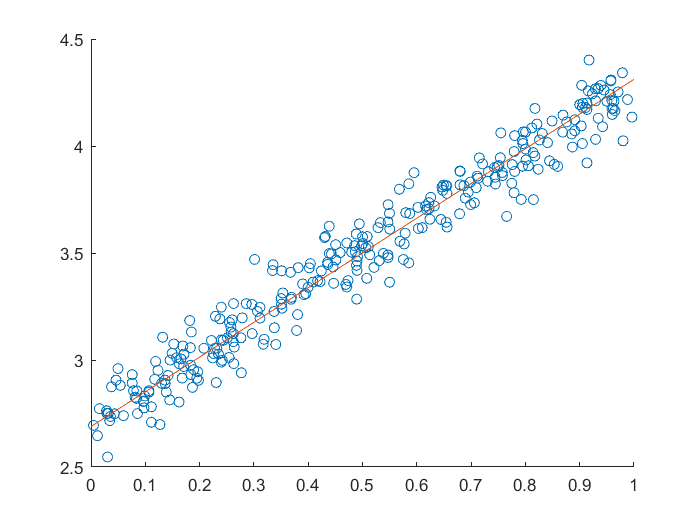
\includegraphics[width=0.5\textwidth]{../results/3/problem3-1.png}
		\caption{The first sample set of points}
	\end{figure}

	As for the second set of points the output generated is
	\begin{figure}[h]
		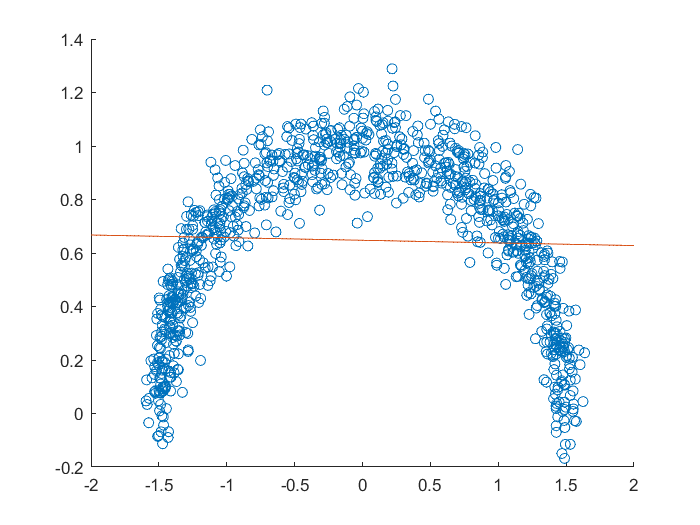
\includegraphics[width=0.5\textwidth]{../results/3/problem3-2.png}
		\caption{The second sample set of points}
	\end{figure}

	Note that for the first data set the eigenvalues turn out to be $0.0025$ and $0.2925$. One eigenvalue is more than 100 times the other. While for the second data set, the eigenvalues turn out to be $0.0957$ and $1.1321$ where the larger is only around 12 times the smaller. Thus, in the second case the linear relationship for $Y$ and $X$ is not as accurate as the one in the first case.

	\newpage
	\section{Problem 4}
	On running the attached code (which takes an eternity to run btw), one finds that the nubmer of ``large'' eigenvalues for every digit is around 8. This is (probably) attributed to the fact that the training set contains digits which are written in similar fashion, and hence, there are not many significant modes of variation.

	Finally, the images that I have put in the folders are from left to right as $\mu$, $\mu - \lambda_1v_1$ and $\mu + \lambda_1v_1$.

	Finally, to answer the last question, take the number 1 for example, we see that the most prominent principal axis is along the line which is almost vertical and hence 1 is written as a vertical line (generally).
	
	\newpage
	\section{Problem 5}
	The logic is as such: We first find the covariance matrix for each digit. Then, we find the eigenvalues and eigenvectors for the same and pick the 84 largest eigenvalues and corresponding eigenvectors, which would be orthogonal. We shall consider these eigenvectors to be our basis for the hyper plane. Finally, we need only find the projection of the required image vector ($\mathbf{x}$) on each of these 84 eigenvectors which is equivalent to finding the dot product of each eigenvector with the image vector.

	For the sake of simplicity, for each digit, I took the image vector to be the mean image vector. In that case, it becomes easier to compare. At this point I must admit that some of the digits don't really look like digits after dimension reduction.

	\newpage
	\section{Problem 6}
	Finding the mean is easy enough and routine computation.


	For the next part, I shall use \href{https://www.cs.uoi.gr/~cnikou/Courses/Image_Analysis/08_PCA_and_Eigenfaces.pdf}{this} text as a reference, since it deals with almost the same problem. The main formula that one would use is:
	\begin{equation*}
		\begin{bmatrix}
			w_1 & w_2 & \cdots & w_k
		\end{bmatrix}
		^T
		= 
		\begin{bmatrix}
			u_1^T \\ u_2^T \\ \vdots \\ u_k^T
		\end{bmatrix}
		(x - \mu)
	\end{equation*}
	where $w_1,w_2,\cdots,w_k$ are the coordinates in the dimension changed space and $u_1,u_2,\cdots,u_k$ are the eigenvectors corresponding to the $k$ largest eigenvalues in decreasing order.

	The idea behind the algorithm is to first shift the mean of all the images to the origin of the space. Then, by considering the top $k$ principal modes of variation, we get the eigenvectors that are required for the dimension reduced space. The first equation that you see on this page is basically taking the dot product of the shifted image vector with each eigenvector since they form the basis of the reduced space to get the corresponding coordinates of the image in the reduced space. Once you get the first equation, the second equation just exploits the fact that $u_i$ are orthonormal.

	Then in order to reconstruct the original image, we use the following formula
	\begin{equation*}
		x = \mu + 
		\begin{bmatrix}
			u_1 & u_2 & \cdots & u_k
		\end{bmatrix}
		\begin{bmatrix}
			w_1 \\ w_2 \\ \vdots \\ w_k
		\end{bmatrix}
	\end{equation*}
	In the context of the problem, the value of $k$ is $4$.

	For generating the random fruit images, I used $\sqrt{\lambda_i}\mathsf{rand()}$ as the weight for each eigenvector.\footnote{This was done since using only $\mathsf{rand()}$ was giving a black image}. The three fruits generated are:
	\begin{figure}[h]
		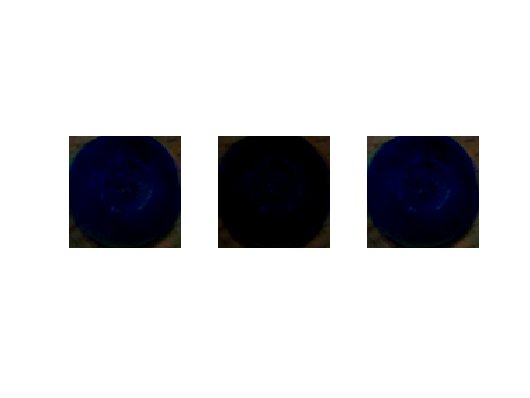
\includegraphics[width=0.5\textwidth]{../results/6/problem6-c.png}
		\caption{The three randomly generated fruits}
	\end{figure}
\end{document}